\subsection{Background}
The most popular type of wearable in 2019 is the smartwatch \cite{best_watches}. 
Smartwatches are devices worn on one's wrist, equipped with sensors, and in some 
cases wireless communication capability for syncing data to a smartphone. They have
rich operating systems (OS), on-board processors and memory, and come in a wide range
of varieties from basic to high-end, with different specialized models in between \cite{smartwatch_arch_rit}.

% ======= TYPICAL SMARTWATCH SPECIFICATIONS =============
\subsection{Typical Specifications}
Modern smartwatches typically have similar components to computers, albeit at a much smaller scale.
They have an OS, which is most cases is proprietary to the manufacturer (i.e. watchOS for Apple);
a single- or dual-core processor ranging from 80MHz to over 1.2GHz depending on the type of watch;
up to a gigabyte of memory; battery life ranging between 18 hours to over a week; and depending on 
the watch - sensors to measure heart rate, fitness statistics, 
and atmospheric pressure \cite{smartwatch_arch_rit}.

It is simple to build a system that can accommodate all the required features of a smartwatch
using normal computing components, however the challenge with a smartwatch is weight, size, and power
consumption, as it needs to fit comfortably on the wrist, and be able to record data for at least
an entire day on a single charge. This means all components must be lightweight, and energy efficient.
As stated earlier in this report, smartwatches are an exploding market, and this is likely due to
advances in hardware allowing high-performance smartwatches at reasonable prices, coming with functions
that are appealing to consumers, driving the demand for this technology. In this report, two different
popular smartwatches will be analyzed.

% ANALYZING APPLE AND GARMIN
\subsection{Analysis of Examples}
Some common examples of smartwatches are the Apple Watch,
and the Garmin Forerunner, both shown below in Figure \ref{watches:pictures}.
These devices are priced quite differently, carry different levels of functionality, and are
targeted towards different segments of the market. Shown below in Table \ref{watch:price} are 
prices for the watches listed above \cite{apple_price} \cite{garmin_price}.

% Figure of all 3 watches
\begin{figure}[h]
    \centering
    \begin{subfigure}{.5\textwidth}
      \centering
      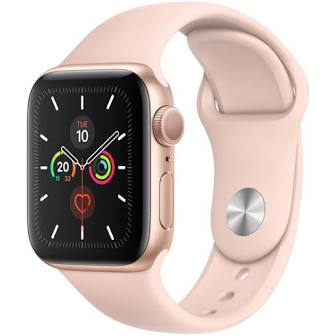
\includegraphics[width=.4\linewidth]{media/apple_pic.jpeg}
      \caption{Apple Watch Series 5 \cite{apple_price}}
      \label{fig:sub1}
    \end{subfigure}%
    \begin{subfigure}{.5\textwidth}
        \centering
        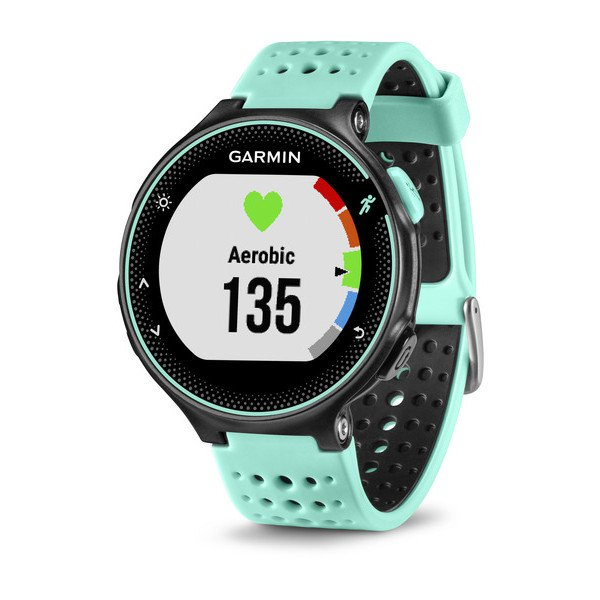
\includegraphics[width=.4\linewidth]{media/garmin_pic.jpeg}
        \caption{Garmin Forerunner 235 \cite{garmin_price}}
        \label{fig:sub3}
      \end{subfigure}
    \caption{Smartwatches discussed in this report.}
    \label{watches:pictures}
\end{figure}

% Watch prices table
\begin{table}[h]
    \centering
    \caption{Smartwatch Prices}
    \csvautotabular{data/prices.csv} 
    \label{watch:price} 
\end{table}

Clearly, these watches come at different price points, target different segments of the market, and
of course come with different architectures for accommodating the necessary features in each model. This
section will cover each of the watches shown above in greater detail.

% ========= APPLE WATCH ===============
\subsubsection{Apple Watch Series 5}
% APPLE WATCH BACKGROUND
\paragraph{Background}
The Apple Watch Series 5 is the newest iteration of smartwatch from Apple Inc., released in September
2019. Priced at \$529, clearly this is considered a higher-end smartwatch, fitting in with Apple's
other product lines (iPhone, iPad, and Mac). This watch has all-day battery life, a touch screen, 
voice call, GPS, compass, and music streaming capabilities, as well as the ability to run thousands of
apps from the Apple App Store, made specifically for the Apple Watch \cite{apple_specs}. This device
is made for Apple users, as it requires an iPhone to make use of all its features.

Much of what makes the Apple Watch quite appealing is the variety of sensor technology that can track
much of your health and fitness data. This sensor technology will be discussed, along with other
computer architecture components in this section.

\paragraph{Hardware}
The processor and System in Package (SiP) at the core of the Apple Watch Series 5 is Apple's S5 chip,
shown below in Figure \ref{fig:s5chip}. This is the fifth iteration of their custom-designed 
smartwatch chip where the entire system is fabricated into a single component \cite{apple_specs}.

% APPLE S5 CHIP FIGURE
\begin{figure}[h]
    \centering
    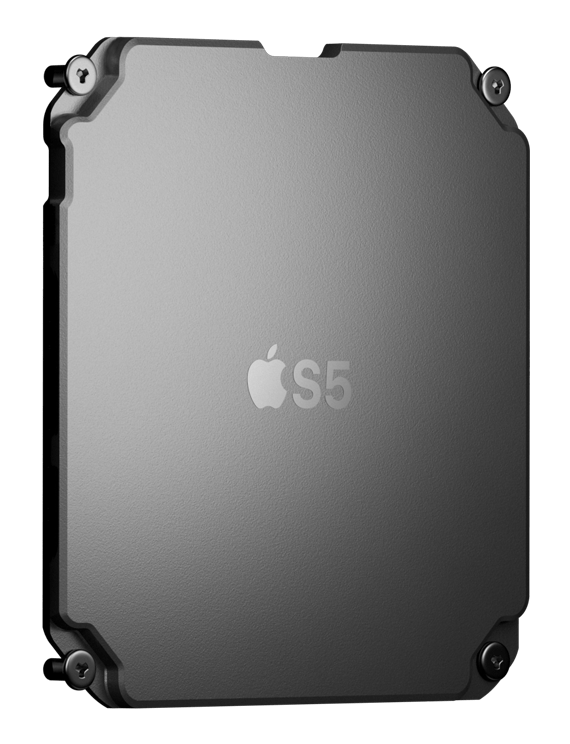
\includegraphics[width=.1\linewidth]{media/apple_s5_chip.png}
    \caption{Apple S5 Processor \cite{apple_s5_pic}}
    \label{fig:s5chip}
\end{figure}

% =========== GARMIN =================
\subsubsection{Garmin Forerunner 235}
If its name wasn't obvious enough, the Garmin Forerunner 235 is first and foremost a runner's
watch.